\chapter{索引构建}
本文从整体上采用滑动窗口机制，也就是索引会有一个窗口生命周期管理，在生成一个新区块时，旧块数据会在索引中删除，新块数据会加入索引。
索引始终维护的是最近窗口大小的数据状态，链尾区块记录的也就是当前索引的最新快照。
\subsection{对象注册}
本文用于集合操作证据生成与验证的密码学累加器对输入全集大小敏感，其证明生成复杂度为 $O(N_1 \cdot N_2)$，其中 $N_1, N_2$ 为输入集 $X_1, X_2$ 的大小。
相较于其他累加器\cite{xu2019vchain}，该方案需以更大的证明来支持交、并、差等嵌套集合操作；
同时，其公钥大小与输入集合元素的全集大小呈二次关系。
由于输入集合的元素来自各滑动窗口中的数据对象，若简单地使用加密散列函数将其编码为 $256$ 位整数，
则公钥规模将达 $(2^{256})^2 = 2^{512}$，显然不可接受。

为解决此问题，我们提出对象注册索引 ObjReg，它为最近 $2^K-1$ 个区块的数据对象分配有限 ID，也为后续属性、范围索引提供了统一标识。
我们强制规定一个最大 ID（记为 $MaxID$），表示跨越 $2^k-1$ 个区块内数据对象的最大可能数量，从而将累加器运算的输入集大小限制在 $MaxID$ 内，进而约束公钥大小。
例如，在实验数据集中将 $MaxID$ 设为 $2^{12}$，则公钥大小被限制为 $(MaxID)^{12} = 2^{24}$。
同时，该机制确保每个连续的 $2^k-1$ 个区块中的数据对象始终具有不同 ID。
如后文所示，我们的集合操作仅涉及 $2^k-1$ 个区块内的数据对象，因此其中每个对象都保证拥有唯一 ID。

ObjReg 是一棵扇出为 $f$ 的完全平衡 Merkle 树，其根哈希写入区块头以承诺以该区块结束的窗口状态，
同时计入区块体供一致性检查。它构建的对象是数据对象的密文摘要：每当数据对象到达，矿工注册该对象，递增计数器并取模 $MaxID$ 来分配其 ID。
由于 ObjReg 具有固定分支，可将 $ID_i$ 视为以 $F$ 为基数的整数，进而得到插入路径：
\[
ID_i = \sum_{j=0}^{h-1} d_j \cdot F^j \quad \text{其中 } d_j \in [0, F-1]
\]
每一位 $d_j$ 对应 ObjReg 第 $j$ 层的子节点选择。因 Merkle 树子节点通常从 $1$ 编号，树路径需取 $d_j+1$。如\ref{fig:objreg} 所示，设扇出 $f=3$，待插入对象 $o_6$ 的 ID 为 $6$，则 $6 = 0\times3^0 + 2\times3^1 + 0\times3^2$，其三进制表示为 $020$，对应树路径为 $(1st, 3rd, 1st)$，即第 $1$、第 $2$ 与第 $1$ 个子节点。

\begin{figure}[h]
    \centering
    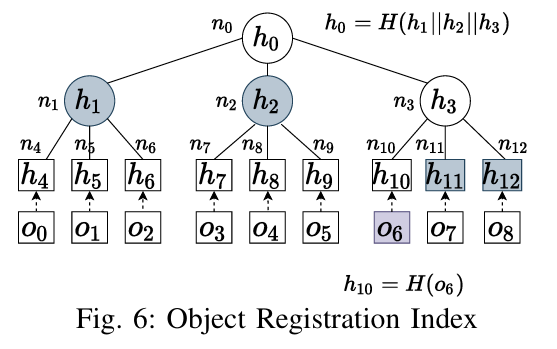
\includegraphics[width=0.5\textwidth]{figures/objreg.png}
    \caption{objreg树}
    \label{fig:objreg}
\end{figure}

从结构上看，ObjReg 是扇出为 $f$ 的完全平衡 Merkle 树，树高取满足 $f^h \ge MaxID$ 的最小值，叶子数为 $f^h$。
每个叶子对应一个 ID 槽位，ID 唯一决定其路径位置，与插入顺序无关。
叶节点定义为 $h_n = H(id \| H(O))$，若该 ID 槽为空则取空摘要；非叶节点定义为子节点哈希的聚合，若为根节点，其哈希值还需绑定当前区块高度。

构建阶段，先对每个对象计算密文摘要，淘汰过时数据后调用 ObjReg 分配唯一 ID,数据可能复用刚过期的 ID，然后将对象摘要写入对应 ID 槽位，
自底向上按扇出 $f$ 计算内部节点，得到子树根哈希。
为确保不同区块高度不会出现相同根哈希，我们将区块高度与子树绑定，生成完整的 ObjReg 根哈希并写入区块头与区块内容。

\section{关键字索引AttDigest}
